\documentclass[xcolor={table}]{beamer}
\usefonttheme{professionalfonts}
\usefonttheme{serif}

\usepackage{times}
\usepackage{tabularx}
\usepackage{ulem}
\usepackage{color,soul}
\usepackage[table]{xcolor}
\usepackage{tikz}
\usetikzlibrary{calc}
\usepackage{graphicx,import}
\usepackage{tcolorbox}

\makeatletter
\newcommand\SoulColor{%
    \let\set@color\beamerorig@set@color
    \let\reset@color\beamerorig@reset@color}
\makeatother

\usetheme{metropolis}           % Use metropolis theme
\title{Multi-Document Summarization: Evaluation, Extraction, and Abstraction}
\date{\today}
\author{Chris Kedzie}
\institute{Dept. of Computer Science, Columbia University}


\begin{document}
  \maketitle


\begin{frame}{Summary Evaluation}
    \begin{figure}
          \small
        \rowcolors{2}{gray!5}{white}
\begin{tabular}{c | c c || c c c c|}
        &  \multicolumn{2}{c||}{Automatic } 
        &  \multicolumn{4}{c|}{Manual } \\
Year & \alert<2>{ROUGE} & \alert<2>{BE} & \alert<2>{Pyramid} & Ling. Quality & Respons. & \alert<2>{Coverage}\\
 \hline 
'01 & & & &X & & X\\
'02 & & & &X & & X\\
'03 & & & &X & X & X\\
'04 & X & & &X & X & X\\
'05 & X & X &X &X &X& \\
'06 & X & X &X &X &X& \\
'07 & X & X &X &X &X& \\
'08 &  &  &X & &X& \\
'09 &  &  &X &X &X& \\
'10 &  &  &X &X &X& \\
'11 &  &  &X &X &X& \\
\hline
\end{tabular}
\end{figure}
\uncover<2>{\alert<2>{*Requires a reference summary}}
\end{frame}

\begin{frame}[t]{\cite{louis2009automatically}}
      \begin{figure}[h]
          \centering
      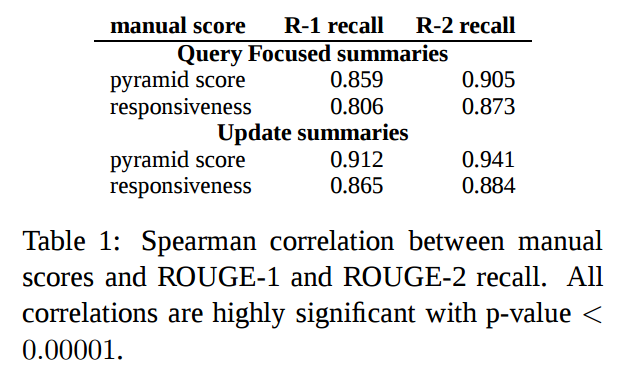
\includegraphics[scale=.25]{images/table1-louis09.png} \\
  \end{figure}
\end{frame}
\begin{frame}[t]{\cite{louis2009automatically}}
      \begin{figure}[h]
          \centering
      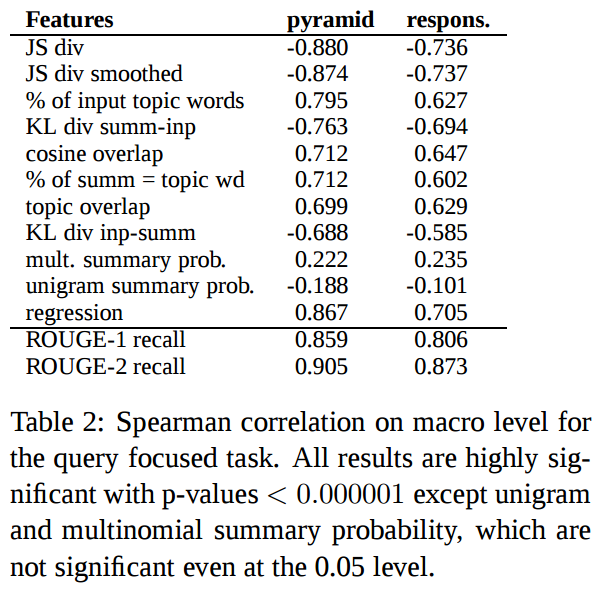
\includegraphics[scale=.25]{images/table2-louis09.png} \\
  \end{figure}
\end{frame}
\begin{frame}[t]{\cite{louis2009automatically}}
      \begin{figure}[h]
          \centering
      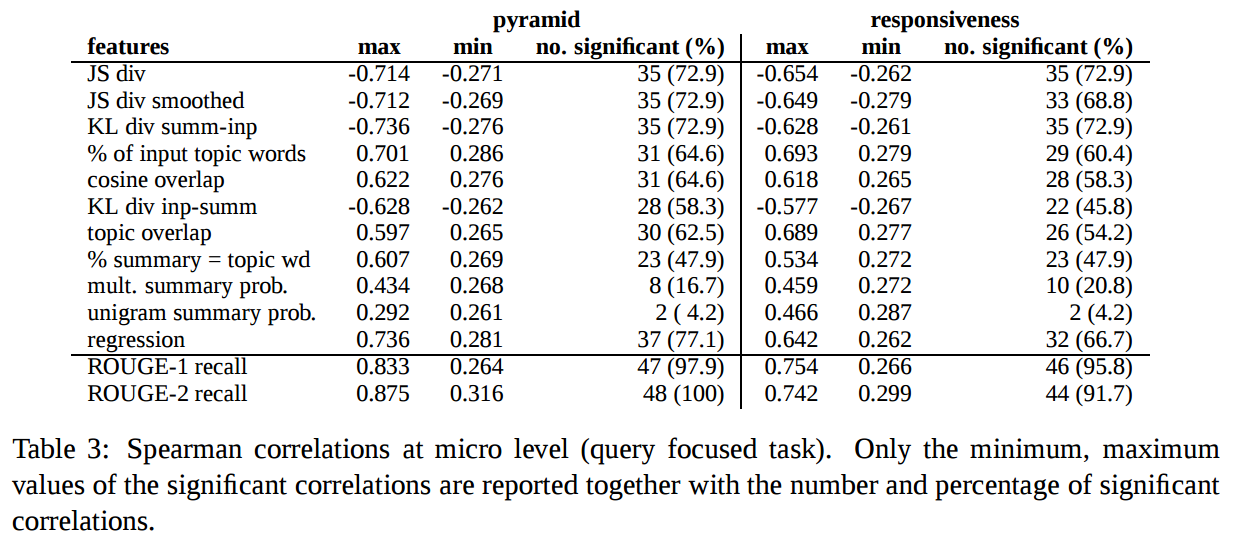
\includegraphics[scale=.25]{images/table3-louis09.png} \\
  \end{figure}
\end{frame}


\begin{frame}[t]{\cite{louis2009automatically}}
      \begin{figure}[h]
          \centering
      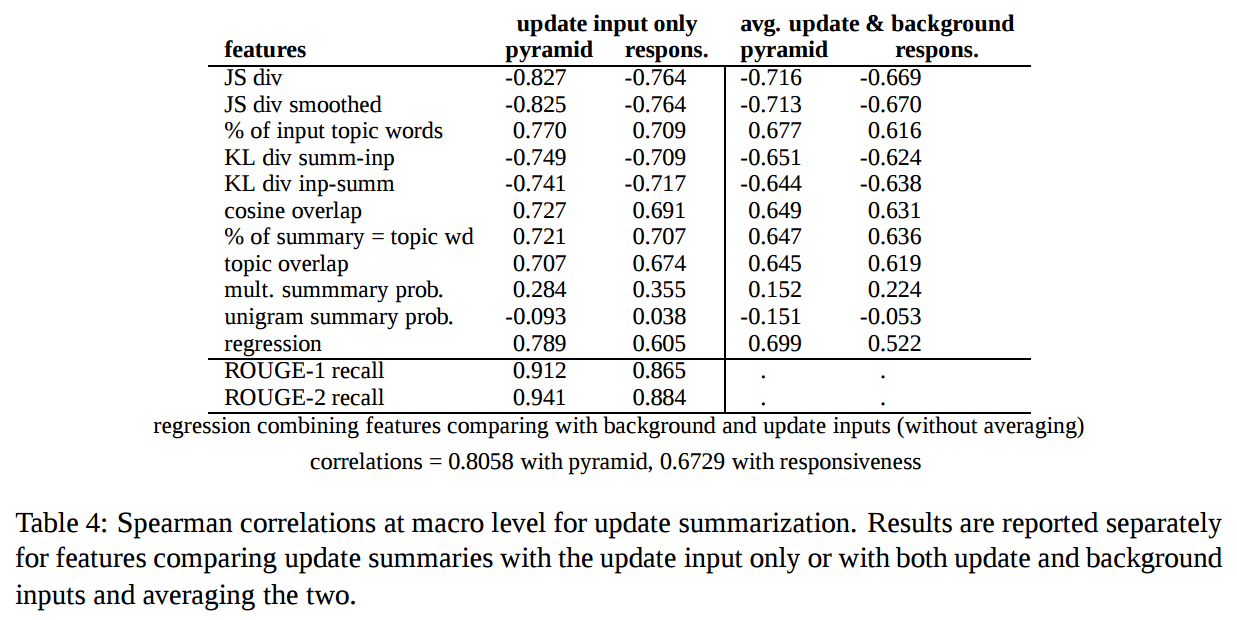
\includegraphics[scale=.25]{images/table4-louis09.png} \\
  \end{figure}
\end{frame}





\begin{frame}[t]{\cite{filippova2008sentence}}
      \begin{figure}[h]
          \centering
      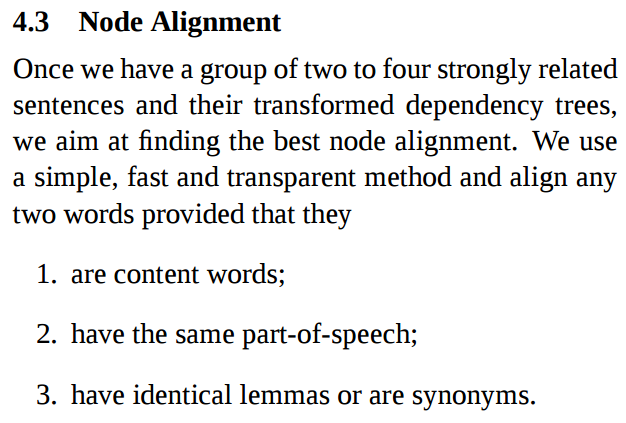
\includegraphics[scale=.25]{images/align-filippova08.png} \\
  \end{figure}
\end{frame}


\begin{frame}[t]{\cite{filippova2008sentence}}
      \begin{figure}[h]
          \centering
          \begin{tabular}{l l}
              objective & 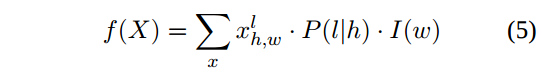
\includegraphics[scale=.25]{images/obj-filippova08.png} \\
              \hline
              structural  &  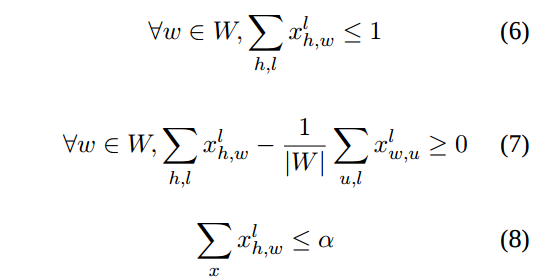
\includegraphics[scale=.25]{images/struct-filippova08.png} \\
              \hline
              allow subordinating clauses &    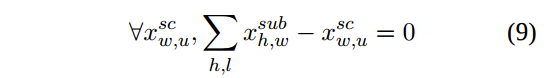
\includegraphics[scale=.25]{images/syn-filippova08.png} \\
              \hline
                                          & 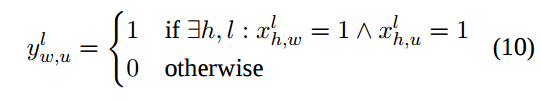
\includegraphics[scale=.23]{images/con-filippova08.png} \\
              semantic agreement &    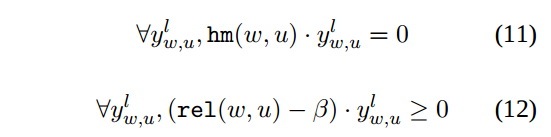
\includegraphics[scale=.23]{images/con2-filippova08.png} \\
                                 &  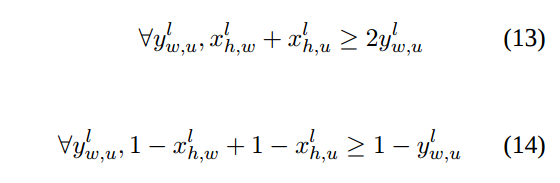
\includegraphics[scale=.23]{images/con3-filippova08.png} \\
          \end{tabular}
  \end{figure}
\end{frame}

\begin{frame}[t]{\cite{filippova2008sentence}}
      \begin{figure}[h]
          \centering
          Syntactic Importance \\
      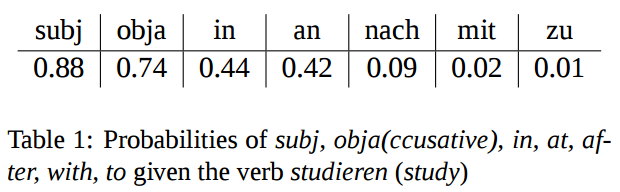
\includegraphics[scale=.25]{images/table1-filippova08.png} \\
      Word Informativeness \\
      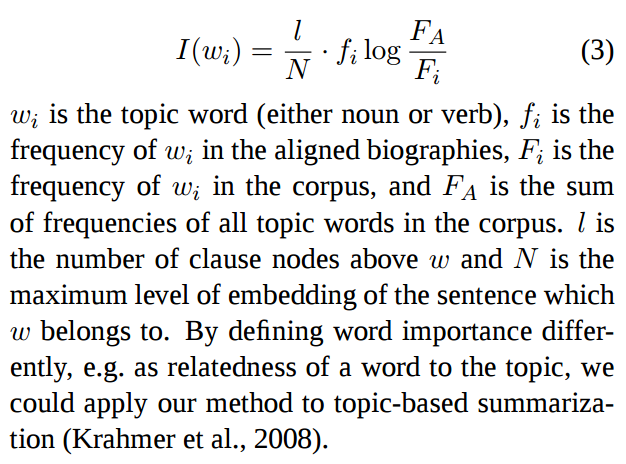
\includegraphics[scale=.25]{images/inf-filippova08.png} \\
  \end{figure}
\end{frame}
\begin{frame}[t]{\cite{filippova2008sentence}}
      \begin{figure}[h]
          \centering
      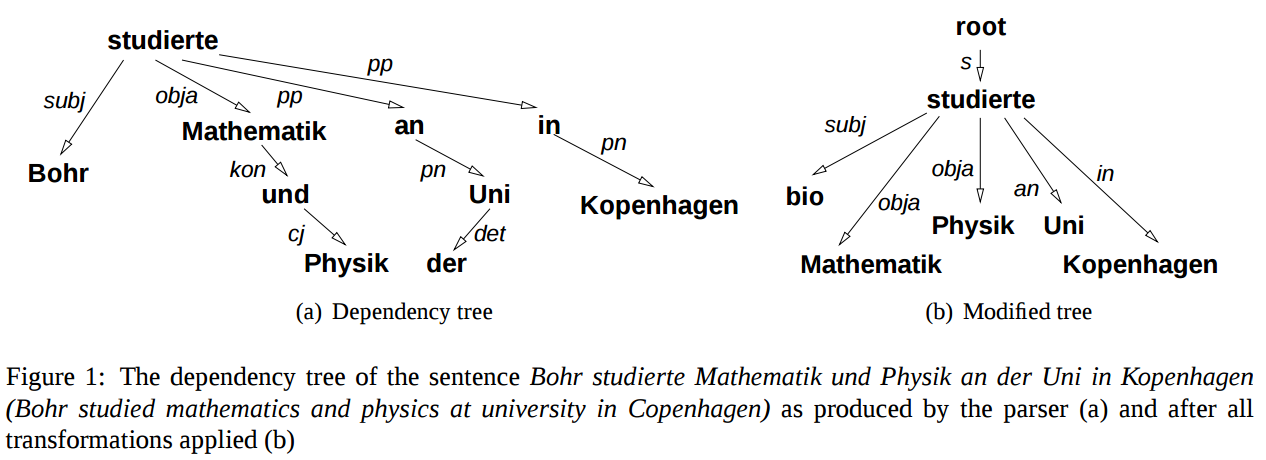
\includegraphics[scale=.25]{images/figure1-filippova08.png} \\
  \end{figure}
\end{frame}
\begin{frame}[t]{\cite{filippova2008sentence}}
      \begin{figure}[h]
          \centering
      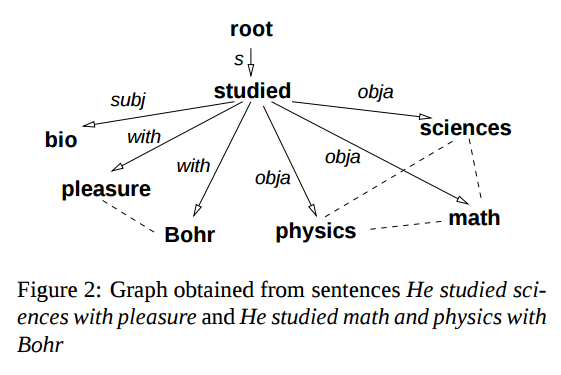
\includegraphics[scale=.25]{images/figure2-filippova08.png} \\
  \end{figure}
\end{frame}
\begin{frame}[t]{\cite{filippova2008sentence}}
      \begin{figure}[h]
          \centering
      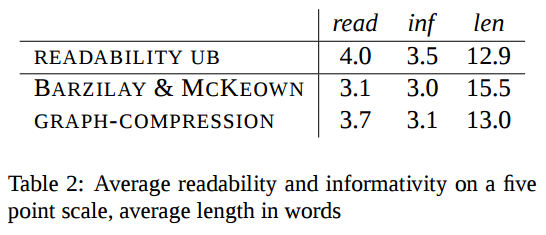
\includegraphics[scale=.25]{images/table2-filippova08.png} \\
  \end{figure}
\end{frame}







\begin{frame}[t]{\cite{martins2009summarization}}
      \begin{figure}[h]
          \centering
      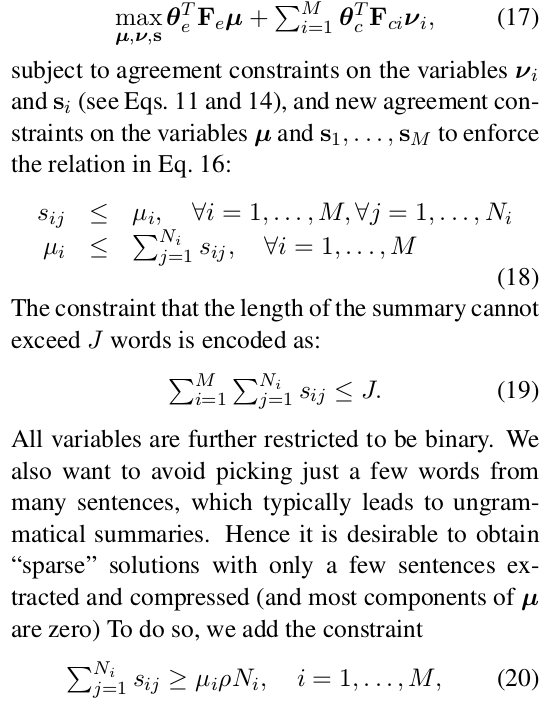
\includegraphics[scale=.25]{images/obj-martins09.png} \\
      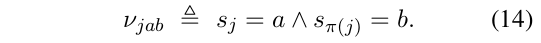
\includegraphics[scale=.25]{images/cons-martins09.png} \\
  \end{figure}
\end{frame}

\begin{frame}[t]{\cite{martins2009summarization}}
    Train compression and extraction weights separately \\
    Data: \textit{compression} Clarke and Lapata, 2008\\
    \textit{extraction} DUC2002 Single Document

    Dependency Features: vars. linear in sentence length $O(N)$ \\
    Bigram Features: vars. quadratic in sentence length $O(N^2)$ \\
~\\
    MIRA is used to learn weights.\\
~\\
    \textcolor{red!70}{Tractability: Non-integer solutions rounded to obtain 
    feasible solution on train and test}\\
        

\end{frame}

\begin{frame}[t]{\cite{martins2009summarization}}
      \begin{figure}[h]
          \centering
      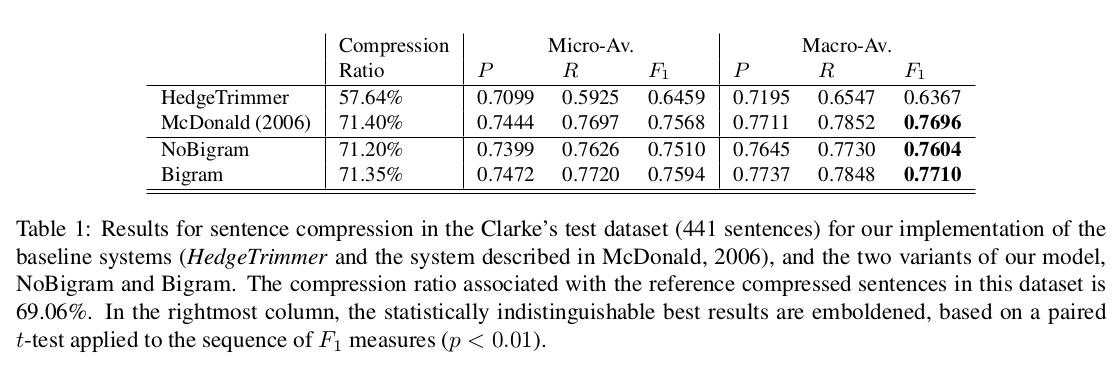
\includegraphics[scale=.25]{images/table1-martins09.png} \\
  \end{figure}
\end{frame}

\begin{frame}[t]{\cite{martins2009summarization}}
      \begin{figure}[h]
          \centering
      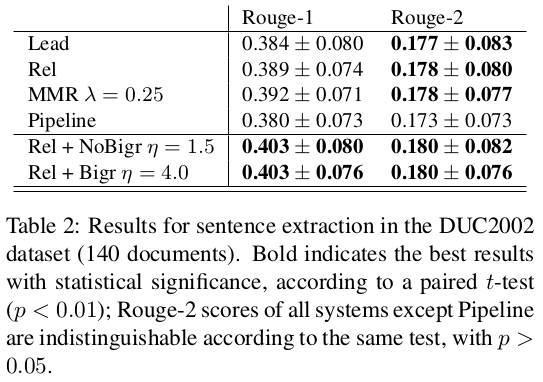
\includegraphics[scale=.25]{images/table2-martins09.png} \\
  \end{figure}

Rel is sentence ranking model using svm, and features:
\begin{itemize}
    \item reciprocal document position
    \item $\mathbf{1}\{\mathrm{is\;lead}\}$
    \item unigram and bigram cosine sim. to title and document
\end{itemize}
~\\
Pipeline is rank, compress, and add until length reached

\end{frame}

\begin{frame}[t]{\cite{berg2011jointly}}
      \begin{figure}[h]
          \centering
      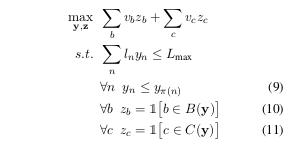
\includegraphics[scale=.7]{images/obj-bergkirkpatrick11.png} \\
  \end{figure}
  $y_n \triangleq$ parse tree node  \\
  $l_n \triangleq$ number of children of $n$th parse tree node  \\
  $v_c \triangleq$ parse tree edge deletion feature score\\
  $v_b \triangleq$ bigram inclusion score\\
  (9) enforces deleting whole subtrees
\end{frame}

\begin{frame}[t]{\cite{berg2011jointly}}
      \begin{figure}[h]
          \centering
      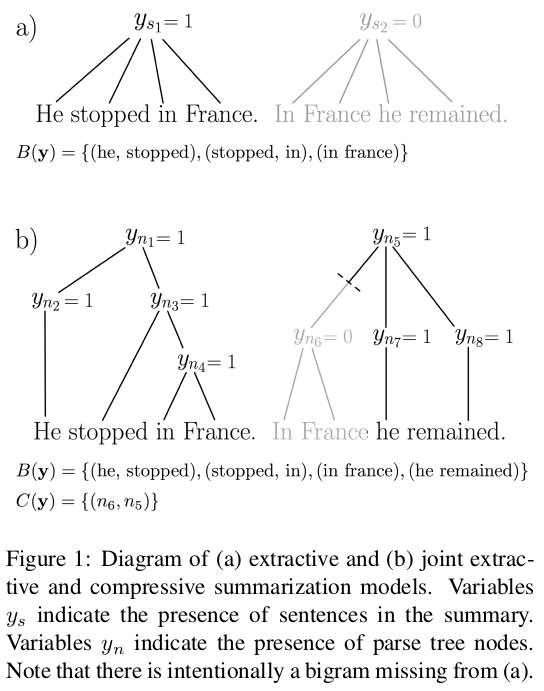
\includegraphics[scale=.29]{images/figure1-bergkirkpatrick11.png} \\
  \end{figure}
\end{frame}
\begin{frame}[t]{\cite{berg2011jointly}}
      \begin{figure}[h]
          \centering
      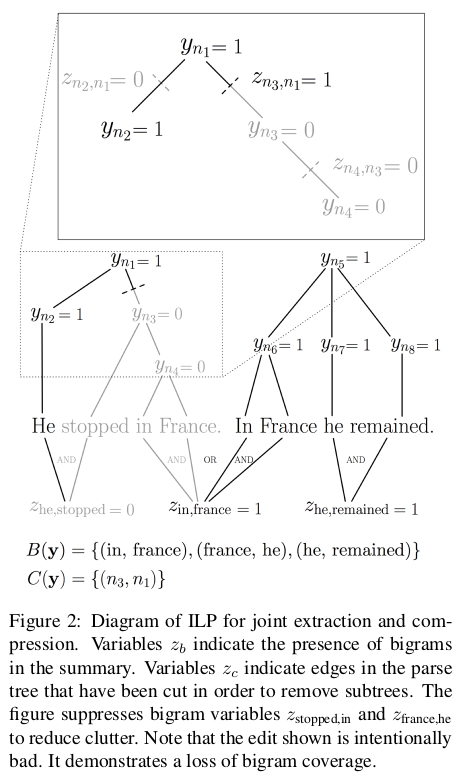
\includegraphics[scale=.29]{images/figure2-bergkirkpatrick11.png} \\
  \end{figure}
\end{frame}


\begin{frame}[t]{\cite{berg2011jointly}}
      \begin{figure}[h]
          \centering
      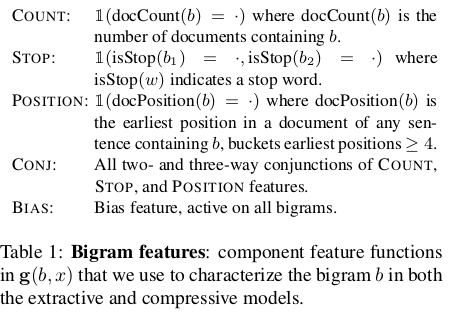
\includegraphics[scale=.27]{images/table1-bergkirkpatrick11.png} 
      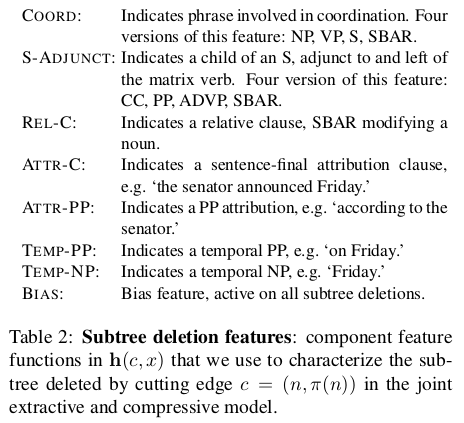
\includegraphics[scale=.27]{images/table2-bergkirkpatrick11.png} \\
  \end{figure}
\end{frame}

\begin{frame}[t]{\cite{berg2011jointly}}
      \begin{figure}[h]
          \centering
      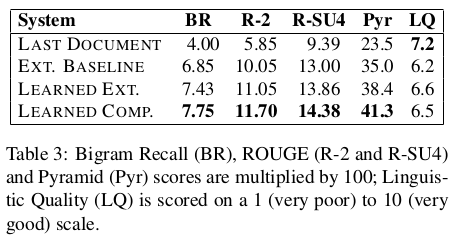
\includegraphics[scale=.29]{images/table3-bergkirkpatrick11.png} 
      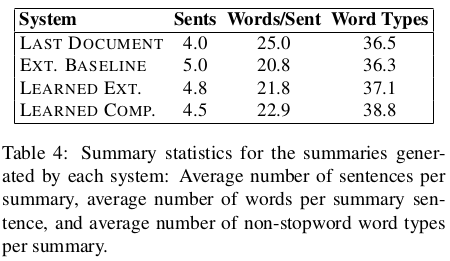
\includegraphics[scale=.29]{images/table4-bergkirkpatrick11.png} 
  \end{figure}
  Results on TAC09 query focused summarization \\
  Decoding done in two phases: 
  \begin{enumerate}
   \item find over-length extractive solution
   \item find compressive solution, fixing extractive solution
  \end{enumerate}

\end{frame}

\begin{frame}[t]{\cite{berg2011jointly}}
      \begin{figure}[h]
          \centering
      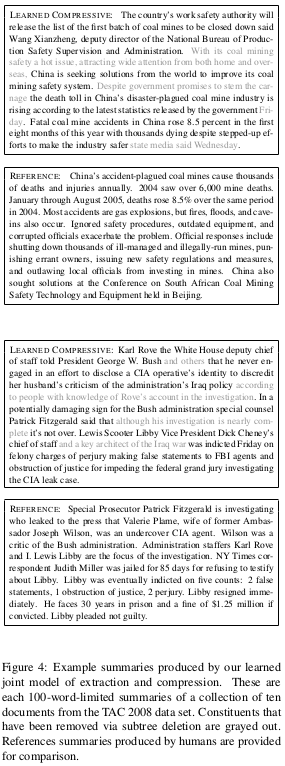
\includegraphics[scale=.29]{images/figure4-bergkirkpatrick11.png} \\
  \end{figure}
\end{frame}



\begin{frame}[t]{\cite{woodsend2010generation}}
      \begin{figure}[h]
          \centering
      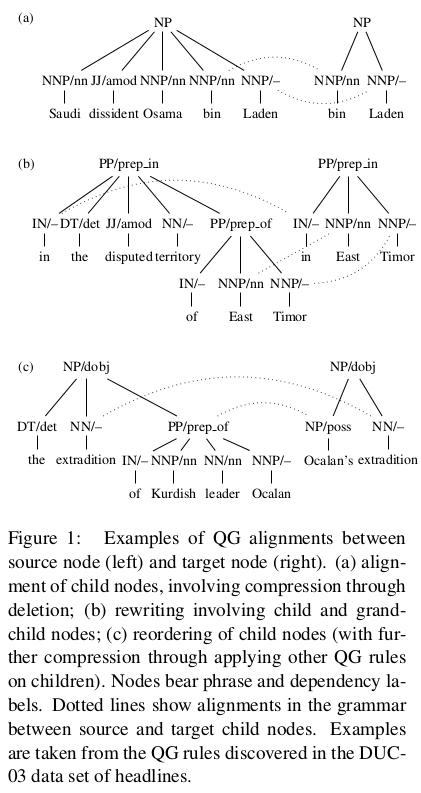
\includegraphics[scale=.25]{images/figure1-woodsend10} 
      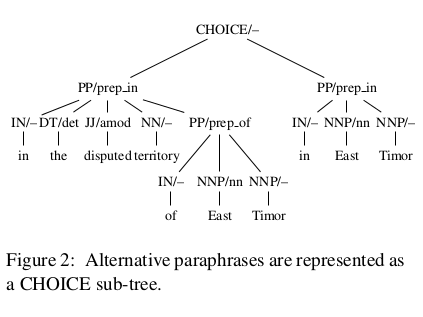
\includegraphics[scale=.25]{images/figure2-woodsend10} 
  \end{figure}
\end{frame}
\begin{frame}[t]{\cite{woodsend2010generation}}
      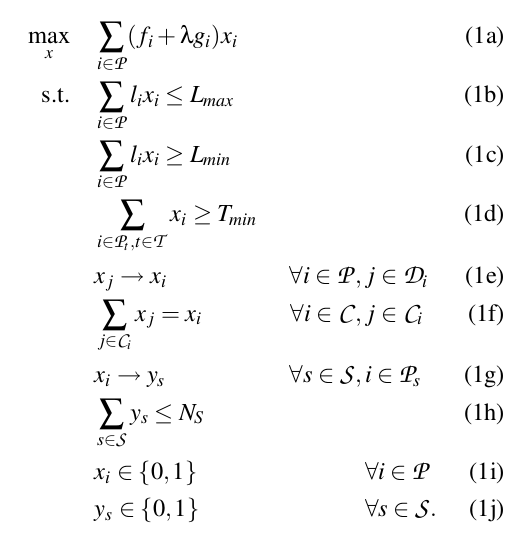
\includegraphics[scale=.23]{images/ilp-woodsend10}  
      \begin{tabular}{p{6.5cm}}
        --- $x_i \triangleq$ phrase nodes\\
        --- $y_i \triangleq$ sentence of the $i$th phrase node\\
        --- $f_i \triangleq$ probability that phrase $i$ has overlap with title  \\
        --- $g_i \triangleq \log \Large( \frac{n_r}{N_r}\Large)$; $\frac{n_r}{N_r} = $ prob. of QG rule\\
        --- 1b -- 1d are length constraints  \\
        --- 1e: if a dependent $x_i$ is kept, $x_i$ must also be kept
        --- 1f: only one child of a choice node is allowed
        --- 1i \& 1j limit number of distinct sentences
        
        

      \end{tabular}

      Features for $f_i$: pos, sentence position, 
        presence of high tf-idf words 
\end{frame}

\begin{frame}[t]{\cite{woodsend2010generation}}
      \begin{figure}[h]
          \centering
      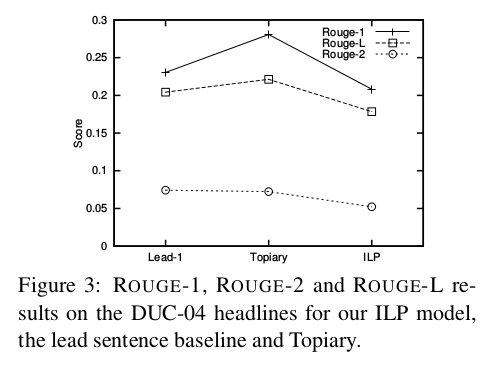
\includegraphics[scale=.25]{images/figure3-woodsend10} \\
      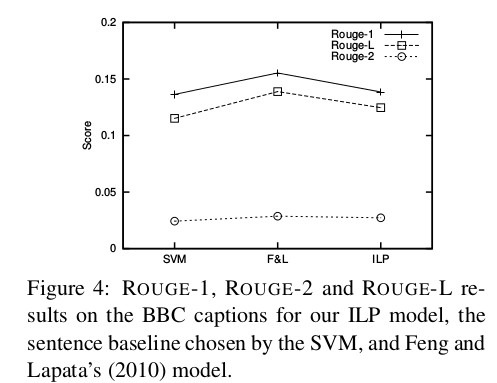
\includegraphics[scale=.25]{images/figure4-woodsend10} 
  \end{figure}
\end{frame}

\begin{frame}[t]{\cite{woodsend2010generation}}
      \begin{figure}[h]
          \centering
      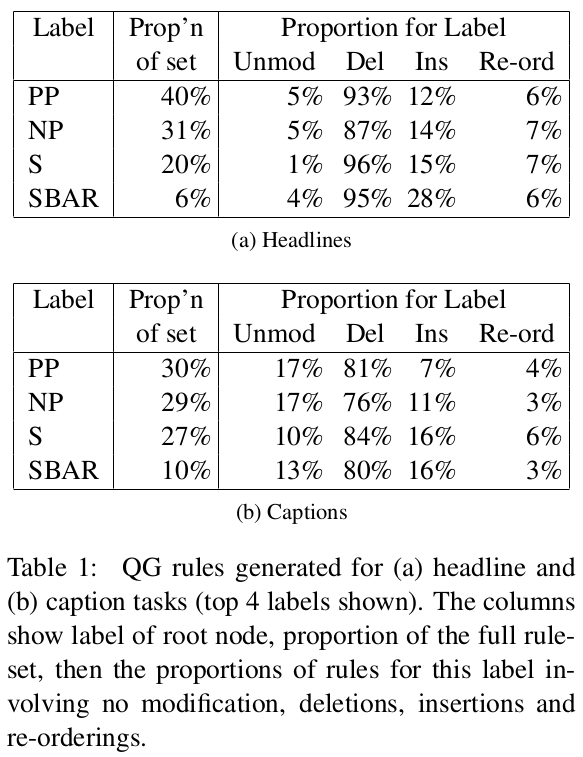
\includegraphics[scale=.25]{images/table1-woodsend10} \\
  \end{figure}
\end{frame}

\begin{frame}[t]{\cite{woodsend2010generation}}
      \begin{figure}[h]
          \centering
      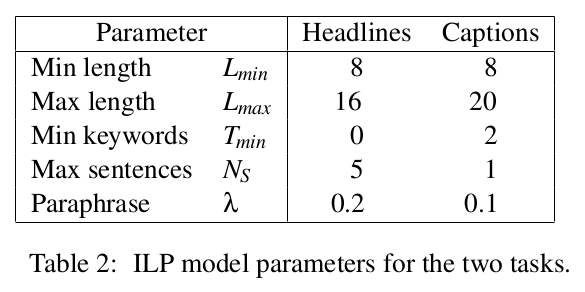
\includegraphics[scale=.25]{images/table2-woodsend10} \\
  \end{figure}
\end{frame}

\begin{frame}[t]{\cite{woodsend2010generation}}
      \begin{figure}[h]
          \centering
      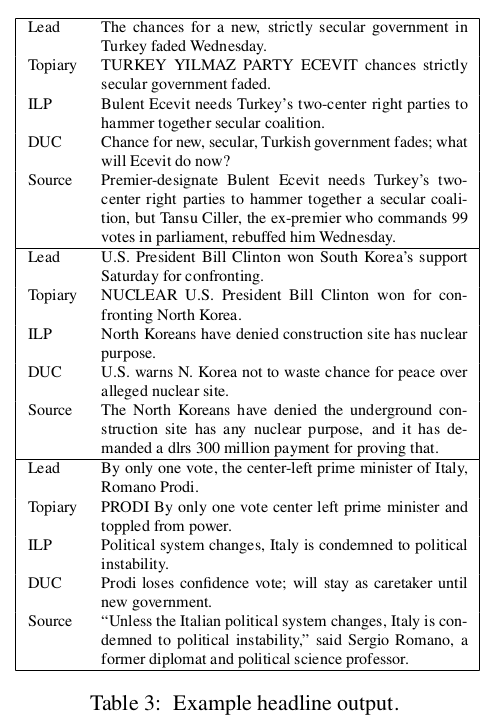
\includegraphics[scale=.25]{images/table3-woodsend10} \\
  \end{figure}
\end{frame}

\begin{frame}[t]{\cite{woodsend2010generation}}
      \begin{figure}[h]
          \centering
      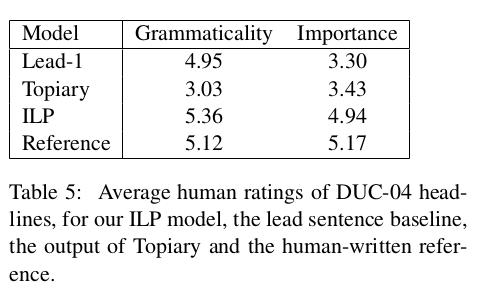
\includegraphics[scale=.25]{images/table5-woodsend10} \\
      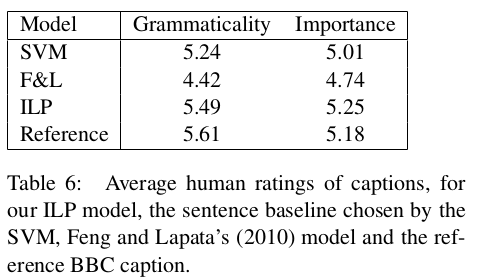
\includegraphics[scale=.25]{images/table6-woodsend10} \\
      \begin{itemize}
              \small
          \item 7 point scale\\ 
          \item ILP significantly better GRAMMATICALITY than topiary\\
          \item ILP significantly better IMPORTANCE than lead\\
      \end{itemize}
  \end{figure}
\end{frame}



\begin{frame}{\cite{wang2013sentence} Sentence Compression}
    Data: Clarke and Lapata, 2008
~\\~\\
    Sequence Based Compression
    \begin{itemize}
        \item CRF over B-Retain, I-Retain, O tag sequences
        \item Rule-based compression applied after finding best tag sequence.
    \end{itemize}
    BASIC Tree Based Compression
    \begin{itemize}
            \small
        \item beam search decoder, with post-order tree traversal
        \item basic scorer: feature based max-ent model over tags 
            $\{Retain, Remove, Partial-Remove\}$ 
    \end{itemize}
\end{frame}
\begin{frame}{\cite{wang2013sentence} Sentence Compression}
    CONTEXT-Aware Tree Based Compression
    \begin{itemize}
            \small
        \item Add contextual prediction features 
    \end{itemize}
    HEAD-driven Tree Based Compression
    \begin{itemize}
            \small
        \item Add contextual prediction features
    \end{itemize}
    Better Beam Rescoring:
    \begin{itemize}
            \small
        \item query relavence
        \item query-independent importance
        \item language model
        \item cross-sentence redundancy
    \end{itemize}    

\end{frame}

\begin{frame}{\cite{wang2013sentence}}
    \begin{figure}[h]
\centering
    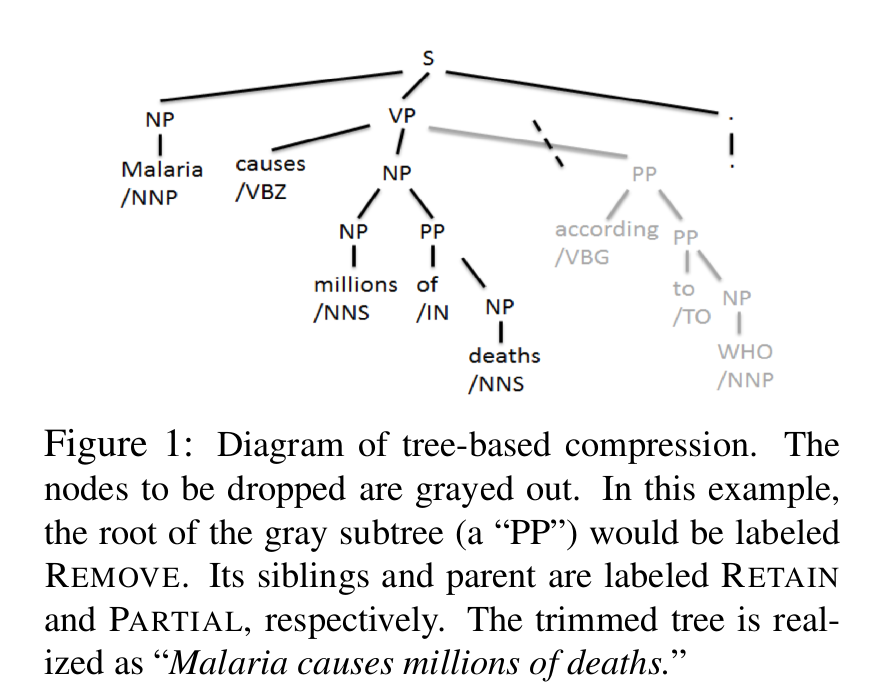
\includegraphics[scale=.27]{images/figure1-wang13} 
\end{figure}
\end{frame}
\begin{frame}{\cite{wang2013sentence}}
    \begin{figure}[h]
\centering
    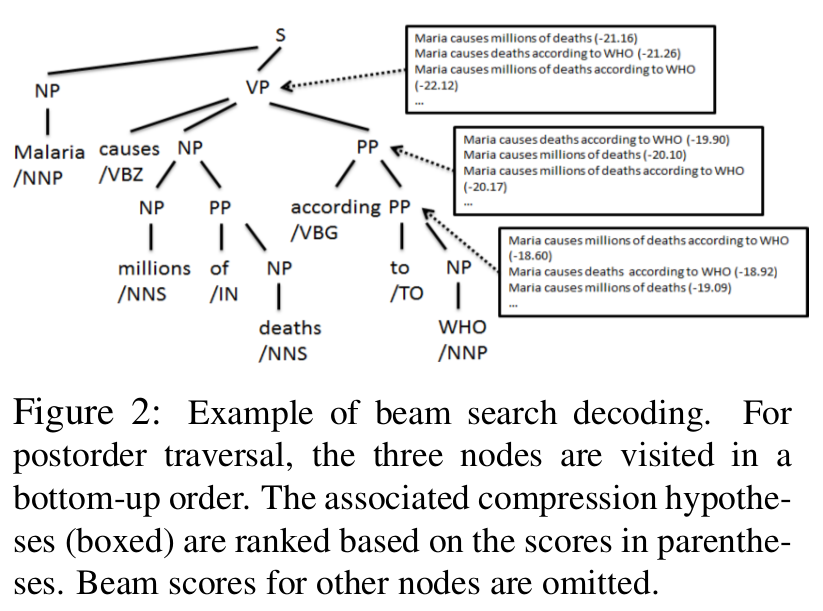
\includegraphics[scale=.3]{images/figure2-wang13} 
\end{figure}
\end{frame}

\begin{frame}{\cite{wang2013sentence}}
\begin{figure}[h]
\centering
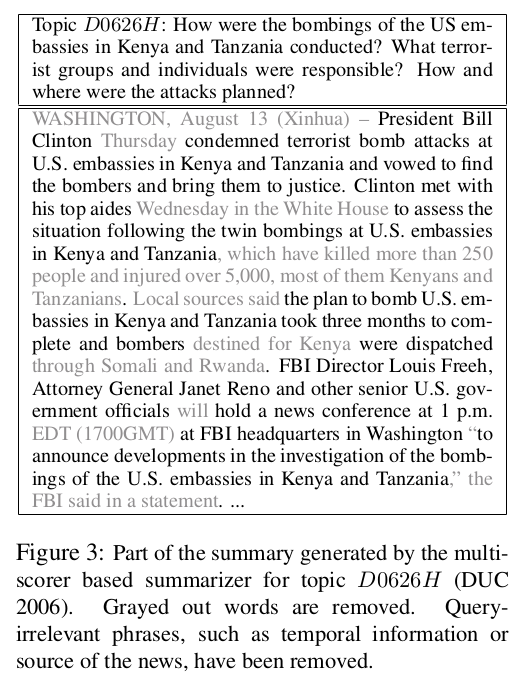
\includegraphics[scale=.27]{images/figure3-wang13} 
\end{figure}
\end{frame}

\begin{frame}{\cite{wang2013sentence}}
\begin{figure}[h]
\centering
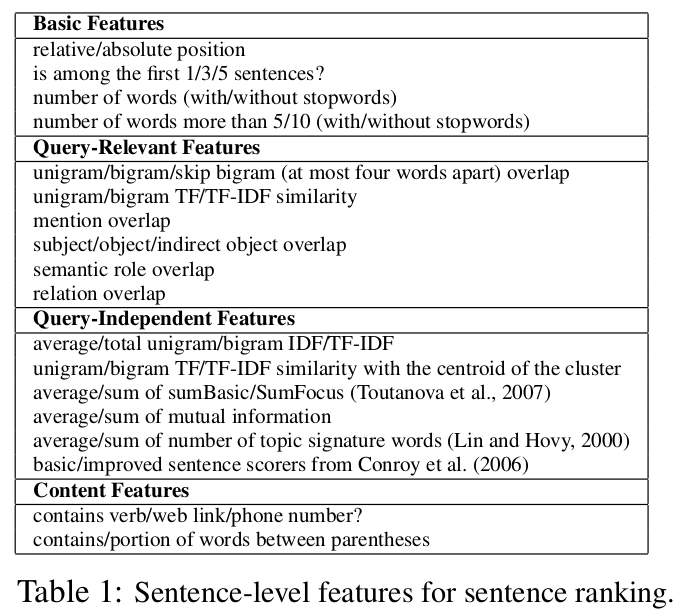
\includegraphics[scale=.3]{images/table1-wang13} 
\end{figure}
\end{frame}

\begin{frame}{\cite{wang2013sentence}}
\begin{figure}[h]
\centering
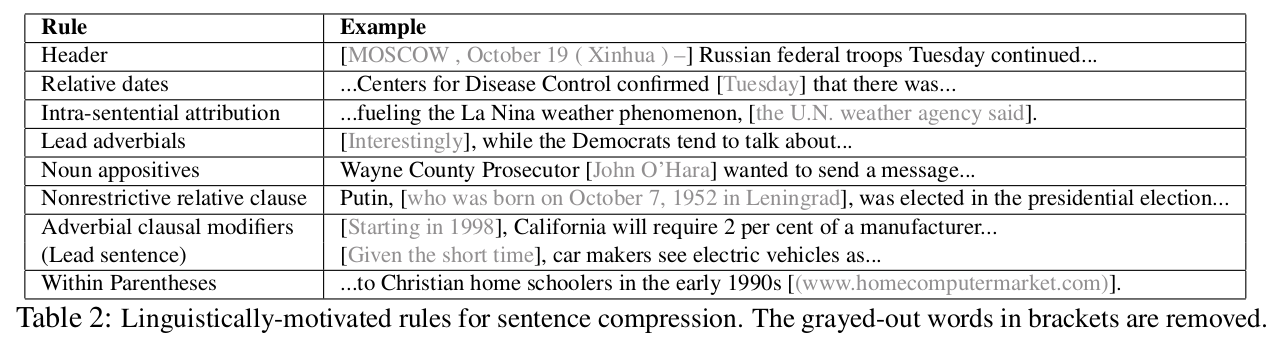
\includegraphics[scale=.22]{images/table2-wang13} 
\end{figure}
\end{frame}

\begin{frame}{\cite{wang2013sentence}}
\begin{figure}[h]
\centering
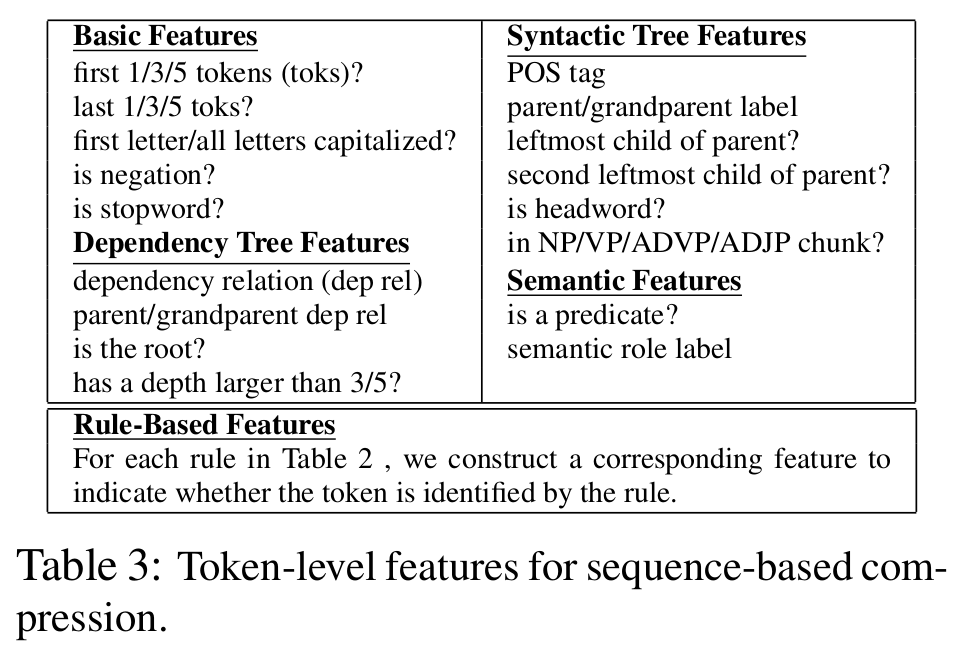
\includegraphics[scale=.3]{images/table3-wang13} 
\end{figure}
\end{frame}

\begin{frame}{\cite{wang2013sentence}}
\begin{figure}[h]
\centering
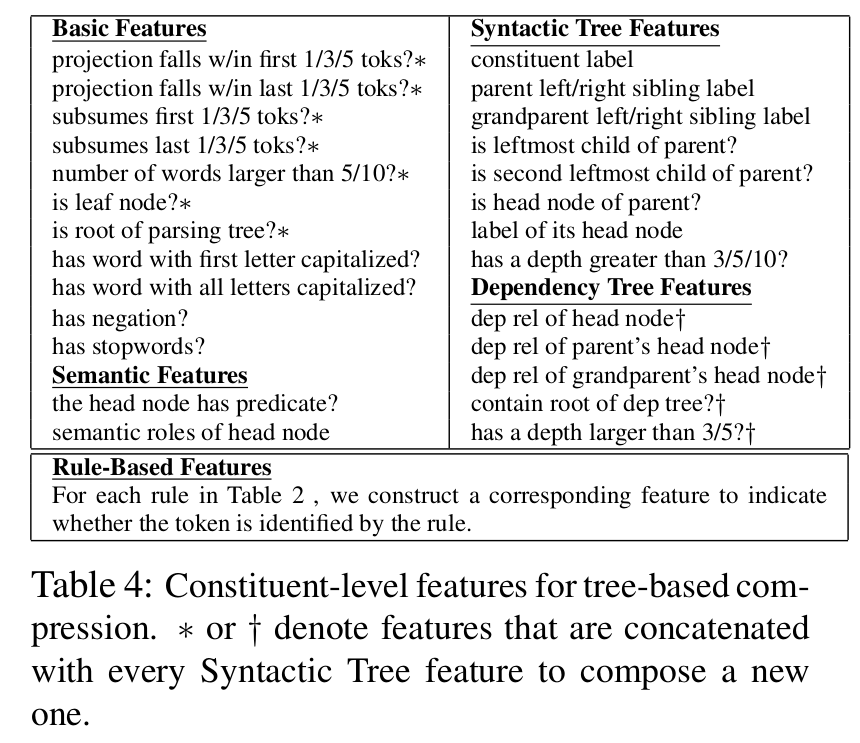
\includegraphics[scale=.25]{images/table4-wang13} 
\end{figure}
\end{frame}

\begin{frame}{\cite{wang2013sentence}}
\begin{figure}[h]
\centering
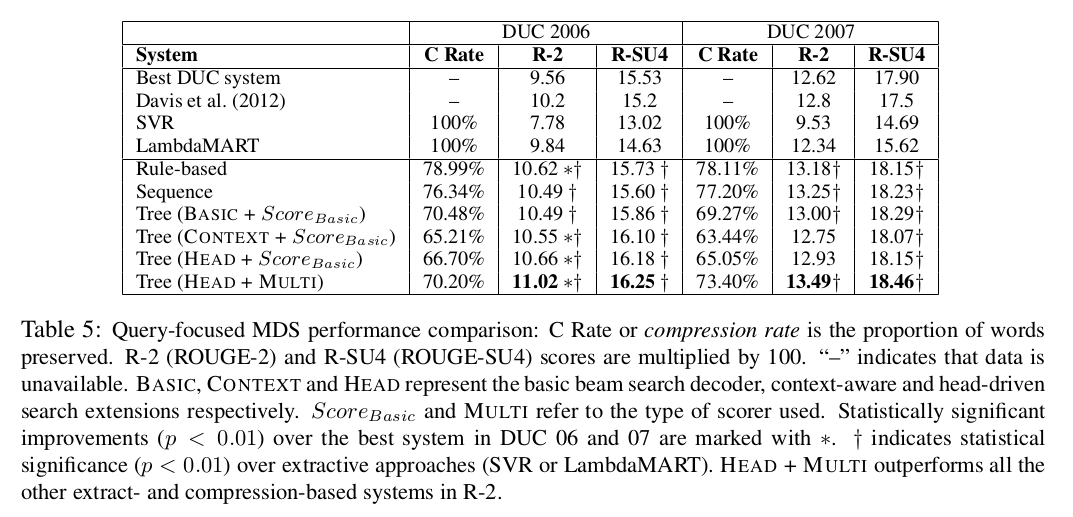
\includegraphics[scale=.27]{images/table5-wang13} 
\end{figure}
\end{frame}

\begin{frame}{\cite{wang2013sentence}}
\begin{figure}[h]
\centering
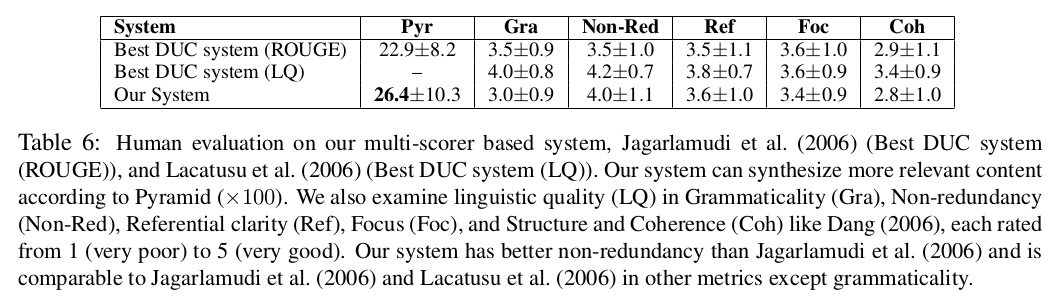
\includegraphics[scale=.27]{images/table6-wang13} 
\end{figure}
\end{frame}

\begin{frame}{\cite{wang2013sentence}}
\begin{figure}[h]
\centering
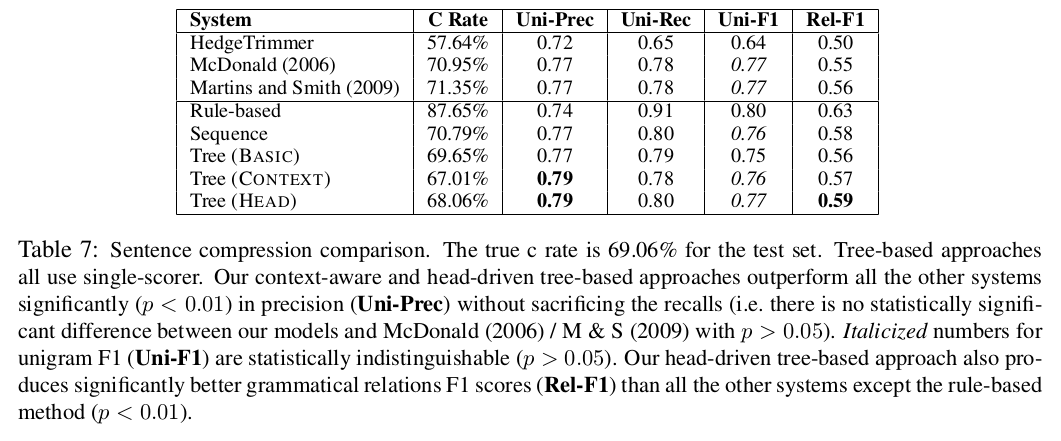
\includegraphics[scale=.27]{images/table7-wang13} 
\end{figure}
\end{frame}

\begin{frame}{\cite{wang2013sentence}}
\begin{figure}[h]
\centering
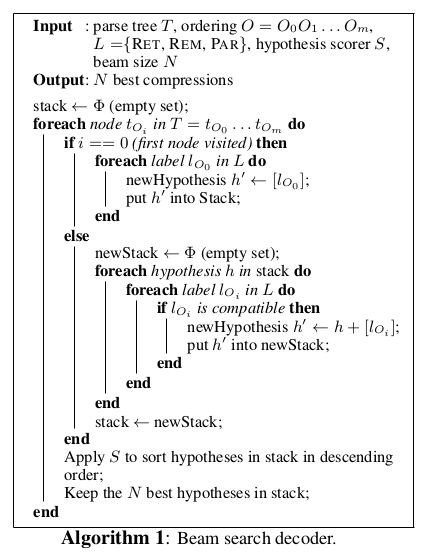
\includegraphics[scale=.3]{images/algo1-wang13} 
\end{figure}
\end{frame}


\bibliographystyle{apalike}
\bibliography{references}


\end{document}

